\documentclass[12pt]{scrartcl}

\usepackage{graphicx}
\graphicspath{./}

\title{Aufgabe 2 --- Oma's Weihnachtskarten}
\subtitle{Theorethische L\"osung}
\author{Julius Makowski}
\date{}

\begin{document}
  \maketitle

  \section{Ansatz}
    Mein Ansatz in dieser Aufgabe ist, das Seniorenheim beziehungsweise die Einwohner*innen als gerichteter, gewichteter Graph darzustellen. Dabei wird jede*r Einwohner*in als Knoten, jeder m{\"o}gliche Weg als Kante betrachtet. Die Beispielaufgabe k{\"o}nnte in der Darstellung so aussehen:

    \vspace{12pt}
    \begin{center}
      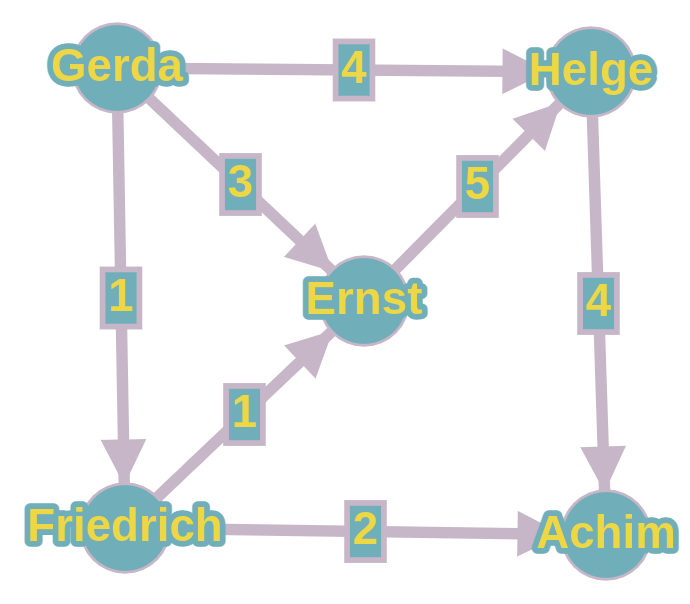
\includegraphics[scale=0.2]{graph}
    \end{center}

    \vspace{12pt}\noindent
    Gesucht ist dann das gesamte Gewicht der \textit{Minimum Spanning Arborescence} -- dem k{\"u}rzesten Weg zu allen Knoten, ausgehend von einem gegebenen Knoten -- in diesem Fall Gerda. Ein Darstellung von dieser k{\"o}nnte so aussehen:

    \vspace{12pt}
    \begin{center}
      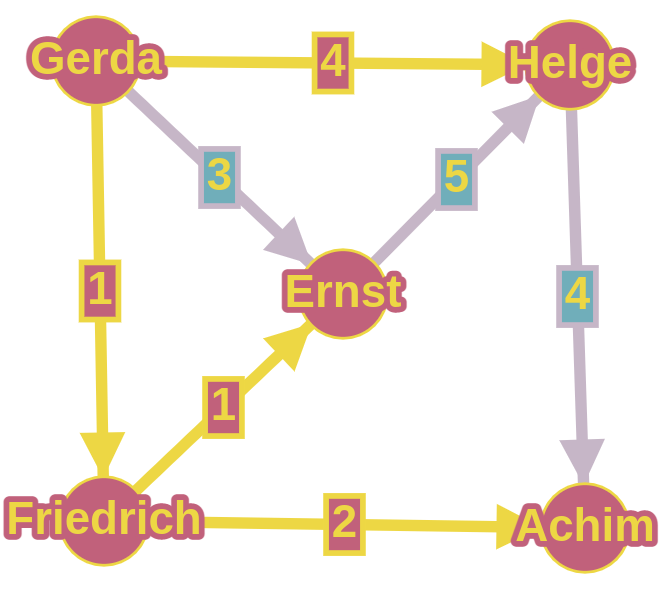
\includegraphics[scale=0.2]{graph_solved}
    \end{center}


  \section{L{\"o}sung}
    Zuert muss eine Datenstruktur gew{\"a}hlt werden, in der Graphen gut dargestellt werden k{\"o}nnen. Dabei habe ich mich f{\"u}r eine Adjazenzliste / Nachbarschaftsliste entschieden. In dieser werden in beliebiger Reihenfolge alle Kanten des Graphen mit dem jeweiligen Gewicht gespeichert.

    \vspace{12pt}\noindent
    Das Implementieren eines Algorithmus zum l{\"o}sen dieser Aufgabe wird schon etwas kniffliger. Der einzige effiziente Algorithmus, der in Frage kommt, ist \textit{Edmond's Algorithm}, der allerdings mit einer mir noch unbekannten Datenstruktur (\textit{Skew Heap}) arbeitet.

    \vspace{12pt}\noindent
    Stattdessen habe ich einen ineffizienteren, aber funktionierenden und leichter verst{\"a}ndlichen Brute Force Algorithmus gew{\"a}hlt. Dieser rekursive Algorithmus arbeitet mit den \textit{unite} und \textit{find} Standardoperationen der Union-Find-Struktur.

    \vspace{12pt}\noindent
  

\end{document}
